\documentclass[10pt]{beamer}

%%%
% PREAMBLE FOR THIS DOC 
%%%
%https://tex.stackexchange.com/questions/68821/is-it-possible-to-create-a-latex-preamble-header
\usepackage{/Users/miw267/Repos/csci246_spring2025/slides/preambles/beamer_preamble_for_CSCI246}

\usetikzlibrary{matrix}


%%% TRY TO RESHOW TOC AT EACH SECTION START (with current section highlighted)
% Reference: https://tex.stackexchange.com/questions/280436/how-to-highlight-a-specific-section-in-beamer-toc
\newcommand\tocforsect[2]{%
  \begingroup
  \edef\safesection{\thesection}
  \setcounter{section}{#1}
  \tableofcontents[#2,currentsection]
  \setcounter{section}{\safesection}
  \endgroup
}


%%%% HERES HOW TO DO IT CORRECTLY
% FIRST IN .STY FILE, DO
%\usetheme[sectionpage=none]{metropolis}
% THEN AT EACH SECTION DO
%\begin{frame}{Outline}
%  \tableofcontents[currentsection]	
%\end{frame}



%\setbeamertemplate{navigation symbols}{}
%\setbeamertemplate{footline}[frame number]{}


%%%
% DOCUMENT
%%%

\begin{document}

%\maketitle

%% Title page frame
%\begin{frame}
%    \titlepage 
%\end{frame}





\title{03/10/2025: Inclusion/Exclusion}
\author{CSCI 246: Discrete Structures}
\date{Textbook reference: Sec 19, Scheinerman}

\begin{frame}
    \titlepage 
\end{frame}


\begin{frame}
\footnotesize 
\begin{mygreenbox}[title=Graded Quiz Pickup]
Quizzes are in the front of the room, grouped into four bins (A-G, H-L, M-R, S-Z) by last name. The quizzes are upside down with your last name on the back. Come find yours before, during, or after class.  Only turn the quiz over if it's yours.
\end{mygreenbox} 
\vfill 

%\begin{myredbox}[title=Announcement: How to be sure you're reading the right section]
%\begin{enumerate}
%	\item Check the current version of the syllabus to confirm the reading for the \textbf{next} course meeting sometime during (or after) class.  
%	\item The most current version of the syllabus can always be found at the \href{https://github.com/mikewojnowicz/csci246_spring2025}{course repo}.  
%\end{enumerate}
%\end{myredbox}

\vfill 


\begin{myyellowbox}[title=Today's Agenda]
\begin{itemize}
	\item Reading quiz (5 mins)
	\item Mini-lecture ($\approx$ 20 mins)
%	%
%	\begin{itemize}
%	\footnotesize 
%	\item Review induction 
%	\end{itemize}
%	%
	\item Group exercises ($\approx$ 20 mins)
\end{itemize}

%	Rationale for group exercises: we got shortchanged on time last couple days, and I already did a lot of lectures, so I want you to practice. Next problems quiz will cover relations and functions: Hamkins and 
%	
\end{myyellowbox}
\vfill 

\end{frame}

\begin{frame}[standout]
Reading Quiz
\end{frame}

\begin{frame}

\begin{mygreenbox}[title= Reading Quiz (Inclusion-Exclusion)]
\footnotesize 
\begin{enumerate}
	\item Replace each ? with a + or - to make the equation correct.
	%
	\begin{align*}
	|A \cup B \cup C| = |A| \; ? \; |B| \; ? \; |C| \; ? \;  |A \cap B| \; ? \; |A \cap C| \; ? \; |B \cap C| \; ? \; | A \cap B \cap C|	
	\end{align*}

	\item (True or False.) Consider the length-$k$ lists whose elements are chosen from the set $\set{1,2,\hdots, n}$.  The number of lists which use all of the elements in $\set{1,2,\hdots, n}$ at least once is $n^k$.
	\item (True or False.) Consider the length-$n$ lists whose elements are chosen from the set $\set{1,2,\hdots,n}$ without repetition. A list is called a \textit{derangement} if the number $j$ does not occupy position $j$ in the list for any $j=1,2,\hdots,n$.  The number of derangements is $n!$. 
	\end{enumerate}
\end{mygreenbox}
	
\end{frame}

\begin{frame}[standout]
Feedback on Friday's Quiz 
\end{frame}



\begin{frame}{Problems Quiz (Equiv. Relations, Partitions, Functions)}
\footnotesize 
\begin{figure}[ht]
        \centering
        \includegraphics[width=.6\textwidth]{images/reading_quiz_scores}
   		 \caption{Median Score = 5/8 (62.5\%)}
\end{figure}
\vfill 
\textbf{Notes.}  	
\begin{enumerate}
\item  3 points. Most people got full credit.
\item 2 points.  Many people struggled here.
\item 3 points.  Most people struggled on this one. A common mistake was proving that $R$ was an equivalence relation.
\end{enumerate}
\end{frame}




%
%\begin{frame}[standout]
%Q  \& A on Group Exercises  (Functions)
%\end{frame}


\begin{frame}[standout]
Overview of inclusion-exclusion
\end{frame}


%{
%\setbeamertemplate{background} 
%{
%    \includegraphics[width=\textwidth]{images/dead}
%}
\begin{frame}
\footnotesize 
%    \usebackgroundtemplate{
%\includegraphics[width=\paperwidth,height=\paperheight]{images/dead}
%    }
    
\begin{mygreenbox}[title=The ski lift operator is absolutely vibing]
Out of 40 people ski lift operators at Bridger Bowl,
	\begin{tabular}{p{0.42\textwidth} p{0.48\textwidth}}
	18 like Led Zeppelin; & 7 like Zeppelin and the Dead;\\
	16 like the Grateful Dead; & 5 like the Zeppelin and Taylor; \\
	12 like Taylor Swift; & 3 like the Dead and Taylor; \\
	& 2 like all three\\
	\end{tabular}
How many lift operators don't like any of these performers?
\end{mygreenbox}
\vfill
\begin{myyellowbox}[title=Poll]
Find the problems with the following claims:

\begin{itemize}
	\item \textbf{Claim.} The answer is \# operators - (\# fans Zep + \# fans Dead + \# fans Swift) =40 -(18+16+12).  \pause \textbf{Analysis.}  This gives -6.  So clearly something is wrong.  But what? \pause We subtracted some people \underline{twice} -- e.g. those that like both Zeppelin and the Dead.
	\item  \textbf{Claim.} We have to add back in the people who like two performers. So the answer is  40 -(18+16+12) + (7+5+3). \pause  \textbf{Analysis.} We made the same mistake again! What happened to the 2 students who like all 3 performers?  We subtracted them 3 times at the beginning, and then added them back in 3 times.  So we must subtract them once more. \pause 
\end{itemize}
\end{myyellowbox}
\vfill 
\textbf{Solution}: 40 - (18+16+12) + (7+5+3) - 2 = 7.
\end{frame}
%}

\begin{frame}
\footnotesize 

\begin{mygreenbox}[title=Formulaic solution]
Let $Z$ be the set of lift operators who like Zeppelin, $D$ be the set of lift operators who like the Dead; and $T$ be the set of
lift operators who like Taylor swift. Then the number of lift operators who like at least one of those performers is given by
%
\begin{align*}
| Z \cup D \cup T | &= |Z| + |D| + |T| \\
& -|Z \cap D| - |Z \cap T | - |D \cap T| \\
& + |Z \cap D \cap T|
\end{align*}
Substituting in known values, we find 33 operators like at least one of those performers, and so 7 operators don't like any of them.

\end{mygreenbox}

\vfill \pause 
\begin{myredbox}[title=General formula]

\begin{figure}
\includegraphics[width=\textwidth]{images/inclusion_exclusion.png}
\end{figure}
\end{myredbox}

\end{frame}

\begin{frame}{Why does inclusion-exclusion work?}
\footnotesize
\begin{figure}
\includegraphics[width=\textwidth]{images/inclusion_exclusion_proof}
\end{figure}

Let us form a chart.  The rows are elements and the columns are terms in the formula.
 
\begin{itemize}\footnotesize
\item If an item is not in a set, the entry is blank.
\item If the item is a member of the set, 
	\begin{itemize}\footnotesize 
	\item We put a a $+$ sign if the column label is an intersection of an odd number of sets.
	\item We put a $-$ sign if the column label is an intersection of an even number of sets.
	\end{itemize}
\end{itemize}

\vfill 

\begin{myyellowbox}[title=Poll]
We want to count each element once.  So each row should contain what? \\ 
 \pause Exactly one more $+$ than $-$.
\end{myyellowbox}
	
\end{frame}


\begin{frame}{Why does inclusion-exclusion work?}
\footnotesize
\begin{figure}
\includegraphics[width=\textwidth]{images/inclusion_exclusion_proof}
\end{figure}

Each element $x$ belongs to exactly $k$ sets. And
%
\begin{align*}
\text{the number of $+$s is } &	\binom{k}{1} + \binom{k}{3} + \binom{k}{5} + \hdots \\
\text{the number of $-$s is } &	\binom{k}{2} + \binom{k}{4} + \binom{k}{6} + \hdots 
\end{align*}

If we sum up these (signed) binomial coefficients, we always get exactly 1! 

\vfill 
\begin{myyellowbox}[title=Exercise]
Verify that this is true with three different elements. 
\end{myyellowbox}
\pause 
Why does this property always hold?
\end{frame}

\begin{frame}
\small 
\begin{mygreenbox}[title=\text{Proposition (Scheinerman Exercise 17.15)}]
For any integer $n>0$,
\[ \binom{n}{0} - \binom{n}{1} + \binom{n}{2} - \binom{n}{3} + \hdots \pm \binom{n}{n} =0 \] 
\end{mygreenbox}
\vfill  \pause 
\begin{myredbox}[title=Remark]
Moving all the negative terms over to the right-hand side gives
\[ \binom{n}{0} + \binom{n}{2} + \binom{n}{4} + \hdots = \binom{n}{1} + \binom{n}{3} + \binom{n}{5} + \hdots \]
In other words, \textit{the number of subsets of an $n$-set with an even number of elements is the same as the number of subsets with an odd number of elements}
\end{myredbox}
\vfill  \pause 
\begin{myyellowbox}[title=Group activity (5 minutes)]
Explain why this formula holds. \\
\textbf{Hint:} Revisit some of theorems and propositions from Sec. 17 (Binomial Coefficients).
\end{myyellowbox}


\end{frame}



\begin{frame}{A justification via Pascal's Triangle}
\footnotesize 
\begin{minipage}{.5\textwidth}
\begin{center}
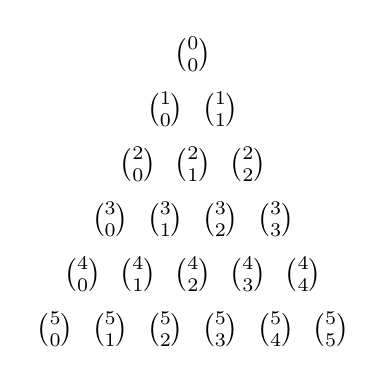
\begin{tikzpicture}[scale=0.7]
\foreach \n in {0,...,5} {
  \foreach \k in {0,...,\n} {
    \node at (\k-\n/2,-\n) {${\n \choose \k}$};
  }
}
\end{tikzpicture}
\end{center}
\end{minipage}
\hfill 
\begin{minipage}{.45\textwidth}
\begin{center}
\includegraphics[width=.95\textwidth]{images/pascals_triangle.png}
\end{center}
\end{minipage}

\vfill 
\begin{myredbox}[title=Remark]
The intermediate number in any row is formed by adding the two numbers just to its left and just to its right in the previous row.
\end{myredbox}
\vfill 
\begin{mygreenbox}[title=\text{Pascal's Identity}]
Let $k$ and $n$ be integers with $0 < k <n$. Then
\[ \binom{n}{k} =\binom{n-1}{k-1} + \binom{n-1}{k} \]
\end{mygreenbox}



\end{frame}


\begin{frame}[standout]
Group exercises
\end{frame}

\begin{frame}
\footnotesize 
\vfill 
\begin{columns}
\begin{column}{0.33\textwidth}
aaron.loomis: 12 \\ 
adam.wyszynski: 17 \\ 
alexander.goetz: 8 \\ 
alexander.knutson: 14 \\ 
anthony.mann: 12 \\ 
blake.leone: 1 \\ 
bridger.voss: 10 \\ 
caitlin.hermanson: 13 \\ 
cameron.wittrock: 13 \\ 
carsten.brooks: 15 \\ 
carver.wambold: 17 \\ 
colter.huber: 7 \\ 
conner.reed1: 1 \\ 
connor.mizner: 10 \\ 
connor.yetter: 11 \\ 
derek.price4: 18 \\ 
devon.maurer: 3 \\ 
emmeri.grooms: 7 \\ 
erik.moore3: 9 \\ 
ethan.johnson18: 4 \\ 
evan.barth: 7 \\\end{column}
\begin{column}{0.33\textwidth}
evan.schoening: 19 \\ 
griffin.short: 20 \\ 
jack.fry: 14 \\ 
jacob.ketola: 13 \\ 
jacob.ruiz1: 2 \\ 
jacob.shepherd1: 21 \\ 
jada.zorn: 4 \\ 
jakob.kominsky: 8 \\ 
james.brubaker: 2 \\ 
jeremiah.mackey: 2 \\ 
jett.girard: 16 \\ 
john.fotheringham: 5 \\ 
jonas.zeiler: 18 \\ 
joseph.mergenthaler: 21 \\ 
joseph.triem: 19 \\ 
julia.larsen: 12 \\ 
justice.mosso: 21 \\ 
kaden.price: 6 \\ 
lucas.jones6: 1 \\ 
luka.derry: 14 \\ 
luke.donaldson1: 15 \\\end{column}
\begin{column}{0.33\textwidth}
lynsey.read: 17 \\ 
mason.barnocky: 3 \\ 
matthew.nagel: 4 \\ 
micaylyn.parker: 5 \\ 
michael.oswald: 20 \\ 
nolan.scott1: 6 \\ 
owen.obrien: 8 \\ 
pendleton.johnston: 5 \\ 
peter.buckley1: 3 \\ 
reid.pickert: 9 \\ 
ryan.barrett2: 11 \\ 
samuel.hemmen: 18 \\ 
samuel.mosier: 11 \\ 
samuel.rollins: 20 \\ 
sarah.periolat: 16 \\ 
timothy.true: 16 \\ 
tristan.nogacki: 19 \\ 
tyler.broesel: 10 \\ 
william.elder1: 6 \\ 
yebin.wallace: 15 \\ 
zeke.baumann: 9 \\\end{column}
\end{columns}
\vfill
\end{frame}


\begin{frame}{Group exercises}
\footnotesize
\begin{enumerate}
	\item A professor in a discrete mathematics class passes out a form asking students to check all the math and computer science courses they have recently taken.  She found that, out of a total of 50 students in the class, 
	
	\begin{tabular}{p{0.42\textwidth} p{0.48\textwidth}}
	30 took precalculus; & 16 took both precalculus and Python;\\
	18 took calculus; & 8 took both calculus and Python; \\
	26 took Python; & 47 took at least one of the three courses; \\
	9 took both precalculus and calculus & \\
	\end{tabular}

	\begin{itemize} \footnotesize 
	\item[a.] How many students did not take any of the three courses?
	\item[b.] How many students took all three courses?
	\item[c.] How many students took precalculus and calculus but not Python? How many students took precalculus but neither calculus not Python?
	\end{itemize}
	\item Of the integers between 1 and 1,000,000 (inclusive), how many are \textit{not} divisible by 2, 3, or 5?
	\item The squares of a 4 $\times$ 4 checkerboard are colored black or white.  Use inclusion-exclusion to find the number of ways the checkerboard can be colored so that no row is entirely one color. 
	\end{enumerate}

\end{frame}




\end{document}
